\section{Introduzione al progetto}

Il progetto che presentiamo in questa relazione ha lo scopo di monitorare il livello dell'acqua in un serbatoio e di avvisare l'utente quando il livello raggiunge una soglia critica. Abbiamo utilizzato la scheda ESP32 Dev Module, integrando il sistema con la piattaforma online Blynk, che ci ha permesso di monitorare in tempo reale i dati raccolti dal sensore di livello dell'acqua e di controllare il sistema di monitoraggio da remoto. Tramite questa piattaforma, abbiamo creato un'interfaccia grafica che visualizza i dati del sensore di livello dell'acqua.    

\subsection{Materiali utilizzati}
Vediamo l'elenco dei materiali che sono stati utilizzati per la realizzazione del circuito:
\begin{itemize}
    \item \textbf{Scheda ESP32 Dev Module\footnote{\mintinline{text}{https://docs.espressif.com/projects/esp-idf/en/latest/esp32/}}:} questa scheda di sviluppo è basata sul microcontrollore ESP32 di Espressif Systems e offre numerose funzionalità, tra cui il supporto per il Wi-Fi e il Bluetooth, un processore a doppio core, una frequenza di clock fino a 240 MHz e numerose interfacce di comunicazione.
    \item \textbf{Sensore ad ultrasuoni per il livello dell'acqua (HC-SR04):} il sensore ad ultrasuoni, noto anche come HC-SR04, è un dispositivo che utilizza ultrasuoni per misurare la distanza da un oggetto. Il sensore invia un segnale sonoro ad alta frequenza (40 KHz) e misura il tempo che impiega il segnale a rimbalzare sull'oggetto e tornare al sensore. La distanza dall'oggetto può essere calcolata conoscendo la velocità del suono nell'aria (circa 343 metri al secondo) e il tempo di volo del segnale. 
    \item \textbf{Mini display OLED:} Il display OLED 128x64 di Arduino è un tipo di schermo a matrice di punti organica a emissione di luce di dimensioni 0,91 pollici con una risoluzione di 128x64 pixel.
    \item \textbf{Buzzer:} Il buzzer è un componente elettronico utilizzato per produrre un suono. Esistono due tipi di buzzer: passivo e attivo. Un buzzer passivo funziona in modo simile ad un altoparlante: vibra e produce un suono quando alimentato con una forma d'onda ad una certa frequenza. Un buzzer attivo, invece, ha integrato un oscillatore interno e produce un suono anche applicando una tensione continua.
    \item \textbf{Pulsante:} I micro pulsanti in dotazione permettono di pilotare ingressi in logica attiva alta (a destra: non premendo si ha \say{0} e premendo si ha \say{1}), mediante resistenza di pull-down, e in logica attiva bassa (a sinistra: non premendo si ha “0” e premendo si ha “1”), mediante resistenza di pull-up
\end{itemize}

\subsection{Schema del circuito}
\begin{figure}[h]
    \centering 
    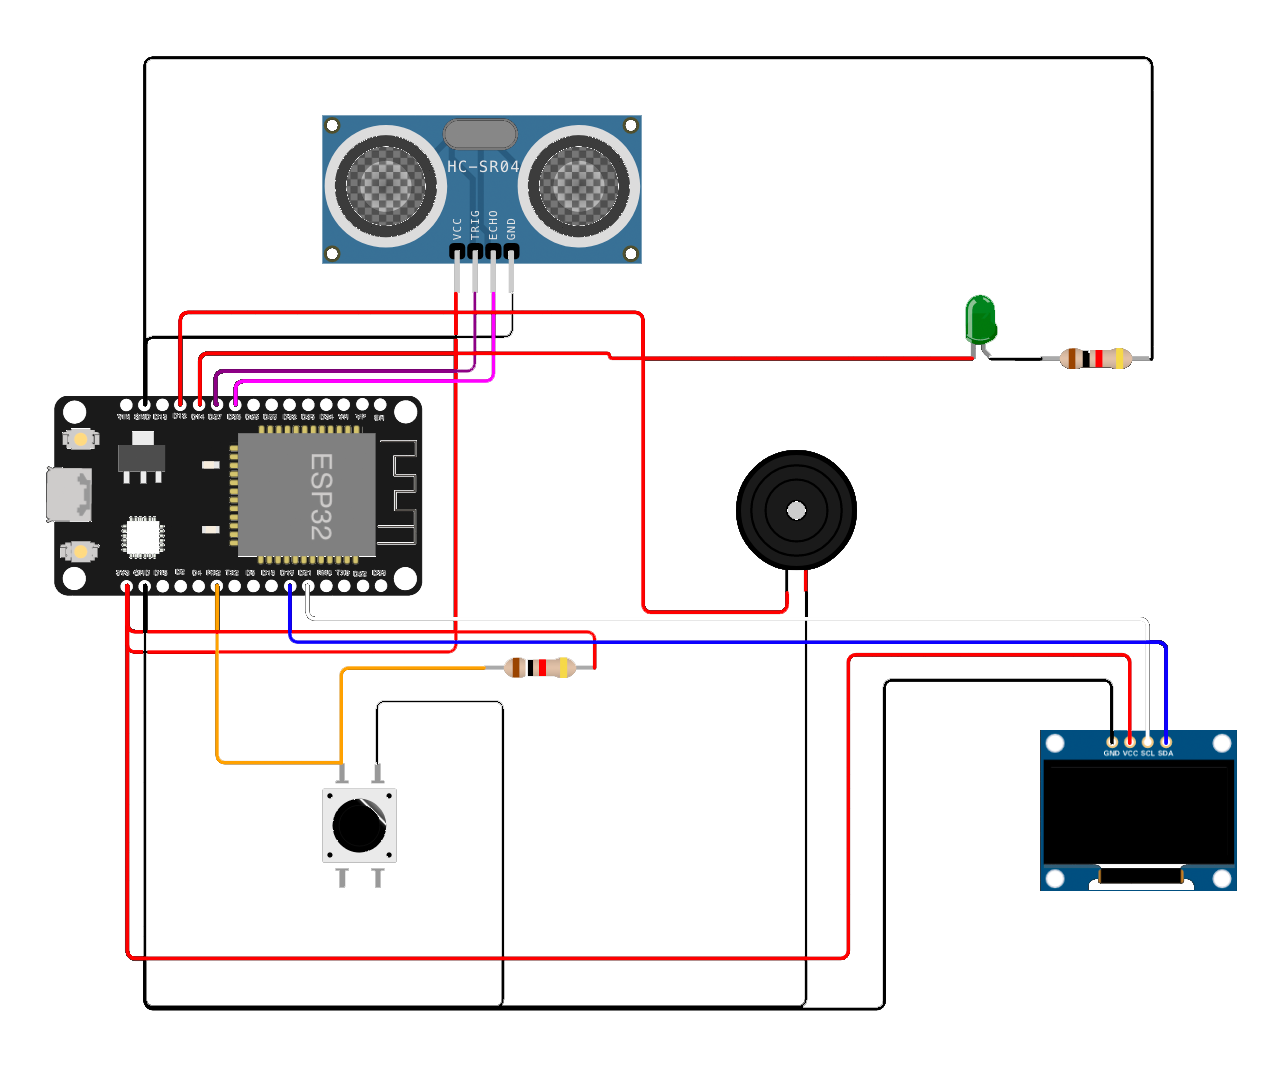
\includegraphics[scale=.6]{img/sketch.png}
    \caption{Schema del circuito.}
    \label{fig:my_label}
\end{figure} 

\section{Implementazione Arduino}

Una volta collegato il circuito con i componenti, abbiamo scritto l'implementazione relativa sull'IDE per Arduino. 

\subsection{Librerie}

Per il funzionamento di tutti i componenti abbiamo importato le librerie necessarie: 

\begin{minted}[tabsize=2,breaklines]{C}
#include <Adafruit_SSD1306.h> 
\end{minted} 

Questa libreria permette di controllare display OLED tramite il controller SSD1306. Adafruit è una società che produce e distribuisce dispositivi elettronici, tra cui anche schermi OLED. Questa libreria fornisce i metodi per inizializzare, scrivere testo e grafica, e controllare l'illuminazione del display.

\begin{minted}[tabsize=2,breaklines]{C}
#include <WiFi.h>
\end{minted} 

Questa libreria fornisce i metodi per connettersi a una rete Wi-Fi tramite un dispositivo ESP32. ESP32 è una famiglia di microcontrollori a basso costo e basso consumo energetico prodotti da Espressif Systems. La libreria WiFi permette di connettersi a una rete Wi-Fi e di inviare e ricevere dati tramite la connessione.

\begin{minted}[tabsize=2,breaklines]{C}
#include <WiFiClient.h>
\end{minted}

Questa libreria è una classe che estende la classe Client e consente di connettersi a un server tramite una connessione Wi-Fi. La classe WiFiClient fornisce i metodi per connettersi a un server tramite un socket TCP/IP e inviare e ricevere dati tramite la connessione.

\begin{minted}[tabsize=2,breaklines]{C}
#include <BlynkSimpleEsp32.h>
\end{minted}

Questa libreria permette di utilizzare il servizio Blynk, un servizio di cloud per dispositivi IoT. Blynk semplifica la connessione di dispositivi IoT a Internet e permette di creare dashboard personalizzate per il monitoraggio e il controllo dei dispositivi. La libreria BlynkSimpleEsp32 fornisce i metodi per inizializzare la connessione a Blynk e per inviare e ricevere dati dalla dashboard.

\begin{minted}[tabsize=2,breaklines]{C}
#include <AceButton.h>
\end{minted}

Questa libreria è una libreria per la gestione di pulsanti su dispositivi embedded. La libreria fornisce un'API per la gestione dei pulsanti, inclusi debounce, ripetizione e gestione di più pulsanti contemporaneamente. La libreria è stata sviluppata per funzionare su una vasta gamma di dispositivi embedded, inclusi microcontrollori a basso costo e a bassa potenza.

\subsection{Implementazione}

\subsubsection{Definizione dei pin scheda ESP32}

Tutti i componenti che abbiamo utilizzato funzianono con un solo pin, tranne nel caso del sensore ad ultrasuoni. Il funzionamento di un sensore ad ultrasuoni inizia con l'invio di un impulso ad alta frequenza dal pin di output del sensore, chiamato pin di trigger. Questo impulso viaggia attraverso l'aria finché non incontra un oggetto. Quando l'impulso incontra un oggetto, viene riflessa e torna indietro verso il sensore. Il sensore ad ultrasuoni utilizza un pin di input, chiamato pin di eco, per rilevare il segnale riflessivo. Il tempo che impiega il segnale ad andare dall'uscita al rientro al sensore è misurato e utilizzato per determinare la distanza dell'oggetto. \\

Nel codice di Arduino, il funzionamento del sensore ad ultrasuoni viene implementato utilizzando una funzione che invia un impulso sul pin di trigger e poi attende il segnale di eco sul pin di eco. La durata del segnale di eco viene quindi utilizzata per calcolare la distanza dell'oggetto.


\begin{multicols}{2}
    \begin{minted}[linenos,tabsize=2,breaklines]{C}
    // Collegamenti al sensore
    #define TRIGPIN    27  // G27
    #define ECHOPIN    26  //G26
    #define wifiLed    2   //G2
    #define ButtonPin1 4  //G4
    #define BuzzerPin  13  //G13
    #define GreenLed   14  //G14
    \end{minted}
    \columnbreak
    La prima riga definisce la costante \mintinline{text}{TRIGPIN} e gli assegna il valore intero 27, che corrisponde al pin di output del sensore per inviare il segnale di trigger. La seconda riga definisce la costante \mintinline{text}{ECHOPIN} e gli assegna il valore intero 26, che corrisponde al pin di input del sensore per ricevere il segnale di eco. 
\end{multicols}
La terza riga definisce la costante wifiLed e gli assegna il valore intero 2, che corrisponde al pin del LED per indicare la connessione WiFi. La quarta riga definisce la costante ButtonPin1 e gli assegna il valore intero 4, che corrisponde al pin del pulsante fisico numero 1. La quinta riga definisce la costante BuzzerPin e gli assegna il valore intero 13, che corrisponde al pin del buzzer. La sesta riga definisce la costante GreenLed e gli assegna il valore intero 14, che corrisponde al pin del LED verde. 

\subsubsection{Implementazione display OLED \mintinline{C}{displayData()}}

\begin{multicols}{2}
\begin{minted}[linenos,tabsize=2,breaklines]{C}
void displayData(int value){
  display.clearDisplay();
  display.setTextSize(4);
  display.setCursor(8,2);
  display.print(value);
  display.print(" ");
  display.print("%");
  display.display();
}
\end{minted}

\columnbreak

La funzione \mintinline{C}{displayData(int value)} viene utilizzata per visualizzare un valore numerico sulla display OLED del dispositivo. In particolare, la funzione riceve in input un valore numerico intero che rappresenta la percentuale di riempimento del serbatoio.
\end{multicols}

\begin{itemize}
    \item Imposta la dimensione del testo a 4 utilizzando la funzione \mintinline{C}{display.setTextSize(4)}.
    \item Posiziona il cursore in una posizione specifica utilizzando la funzione \mintinline{C}{display.setCursor(8,2)}.
    \item Stampa il valore numerico passato in input sulla display OLED utilizzando la funzione \mintinline{C}{display.print(value)}.
    \item Aggiunge uno spazio e il simbolo percentuale al valore numerico stampato utilizzando la funzione \mintinline{C}{display.print(" ")} e \mintinline{C}{display.print("%")}.
    \item Aggiorna la display OLED utilizzando la funzione \mintinline{C}{display.display()}.
\end{itemize}

\subsubsection{Funzione di misurazione}

\begin{multicols}{2}
\begin{minted}[linenos,tabsize=2,breaklines]{C}
void measureDistance(){
  // Set the trigger pin LOW for 2uS
  digitalWrite(TRIGPIN, LOW);
  delayMicroseconds(2);
 
  // Set the trigger pin HIGH for 20us to send pulse
  digitalWrite(TRIGPIN, HIGH);
  delayMicroseconds(20);
 
  // Return the trigger pin to LOW
  digitalWrite(TRIGPIN, LOW);
 
  // Measure the width of the incoming pulse
  duration = pulseIn(ECHOPIN, HIGH);
 
  // Determine distance from duration
  // Use 343 metres per second as speed of sound
  // Divide by 1000 as we want millimeters
 
  distance = ((duration / 2) * 0.343)/10;
\end{minted}

\columnbreak

La funzione measureDistance() viene chiamata all'interno del loop principale e viene utilizzata per misurare la distanza tra il sensore di distanza e l'oggetto che si trova di fronte ad esso.

In particolare, la funzione utilizza un sensore ad ultrasuoni o laser per emettere un impulso acustico e misurare il tempo che impiega a tornare indietro dopo essere stato riflettuto dall'oggetto. Il tempo di viaggio dell'impulso viene quindi utilizzato per calcolare la distanza tra il sensore e l'oggetto. La funzione esegue i seguenti passaggi:

\begin{itemize}
    \item Setta il pin di trigger del sensore a basso per 2 microsecondi.
    \item Setta il pin di trigger del sensore ad alto per 20 microsecondi per inviare un impulso.
    \item Ritorna il pin di trigger a basso.
    \item Misura la durata dell'impulso riflesso dal sensore di distanza tramite la funzione pulseIn().
    \item Calcola la distanza utilizzando la velocità del suono (343 metri al secondo) e la metà della durata dell'impulso, in millimetri.
\end{itemize}

\end{multicols}

Effettua alcune operazioni di controllo sulla distanza misurata, ad esempio verifica se la distanza si trova tra il livello massimo e minimo di riempimento del serbatoio, e calcola la percentuale di riempimento del serbatoio in base alla distanza:

\begin{minted}[tabsize=2,breaklines]{C}
if (distance > (fullTankDistance - 10)  && distance < emptyTankDistance ){
    waterLevelPer = map((int)distance ,emptyTankDistance, fullTankDistance, 0, 100);
    displayData(waterLevelPer);
    Blynk.virtualWrite(VPIN_BUTTON_1, waterLevelPer);
    Blynk.virtualWrite(VPIN_BUTTON_2, (String(distance) + " cm"));

    // Print result to serial monitor
    Serial.print("Distance: ");
    Serial.print(distance);
    Serial.println(" cm");

    if (waterLevelPer < triggerPer){
      digitalWrite(GreenLed, HIGH);
      if (toggleBuzzer == HIGH){
        digitalWrite(BuzzerPin, HIGH);
      }      
    }
    if (distance < fullTankDistance){
      digitalWrite(GreenLed, LOW);
      if (toggleBuzzer == HIGH){
        digitalWrite(BuzzerPin, HIGH);
      } 
    }

    if (distance > (fullTankDistance + 5) && waterLevelPer > (triggerPer + 5)){
      toggleBuzzer = HIGH;
      digitalWrite(BuzzerPin, LOW);
    }        
  }
  // Delay before repeating measurement
  delay(100);
\end{minted}

Invia i dati raccolti alla piattaforma Blynk utilizzando la funzione Blynk.virtualWrite() per visualizzare i dati sulla dashboard Blynk. Accende o spegne un led verde e un buzzer in base alla distanza e alla percentuale di riempimento del serbatoio. Ritorna al loop principale e attende 100 millisecondi prima di eseguire una nuova misurazione.

\subsubsection{Funzione \mintinline{C}{setup()}}

\begin{minted}[tabsize=2,breaklines]{C}
void setup() {
  // Set up serial monitor
  Serial.begin(115200);
 
  // Set pinmodes for sensor connections
  pinMode(ECHOPIN, INPUT);
  pinMode(TRIGPIN, OUTPUT);
  pinMode(wifiLed, OUTPUT);
  pinMode(GreenLed, OUTPUT);
  pinMode(BuzzerPin, OUTPUT);

  pinMode(ButtonPin1, INPUT_PULLUP);

  digitalWrite(wifiLed, LOW);
  digitalWrite(GreenLed, LOW);
  digitalWrite(BuzzerPin, LOW);

  config1.setEventHandler(button1Handler);
  
  button1.init(ButtonPin1);

  if(!display.begin(SSD1306_SWITCHCAPVCC, 0x3C)) {
    Serial.println(F("SSD1306 allocation failed"));
    for(;;);
  }
  delay(1000);  
  display.setTextSize(1);
  display.setTextColor(WHITE);
  display.clearDisplay();

  WiFi.begin(ssid, pass);
  timer.setInterval(2000L, checkBlynkStatus); // check if Blynk server is connected every 2 seconds
  Blynk.config(auth);
  delay(1000);
 
}
\end{minted}

\subsubsection{Funzione \mintinline{C}{loop()}}

\begin{minted}[tabsize=2,breaklines]{C}
void loop() {
  measureDistance();

  Blynk.run();
  timer.run(); 

  button1.check();
}
\end{minted}

\subsection{Integrazione con Blynk}

Blynk è una piattaforma di sviluppo IoT che offre un'ampia gamma di funzionalità per la creazione di applicazioni per dispositivi mobili e il controllo remoto dei dispositivi attraverso Internet. Nel progetto di monitoraggio del livello dell'acqua che abbiamo realizzato, abbiamo utilizzato Blynk per creare un'interfaccia grafica personalizzata che ci ha permesso di visualizzare in tempo reale i dati rilevati dal sensore di distanza ad ultrasuoni e di controllare il buzzer e il pulsante da remoto. \\

Abbiamo utilizzato i pin virtuali di Blynk per collegare i nostri componenti al server Blynk, che ci ha permesso di inviare e ricevere dati in tempo reale tra il nostro dispositivo e la piattaforma Blynk. Abbiamo creato due pin virtuali per il nostro progetto: V1 per visualizzare il livello dell'acqua sul mini display OLED, V2 per attivare o disattivare il buzzer. Questi pin virtuali sono stati utilizzati per comunicare con il nostro dispositivo ESP32 e per inviare comandi attraverso la piattaforma Blynk. 
\begin{multicols}{2}
    \begin{minted}[linenos,tabsize=2,breaklines]{C}
    // Pin virtuali per Blynk
    #define VPIN_BUTTON_1    V1 
    #define VPIN_BUTTON_2    V2
    \end{minted}
    \columnbreak
    Infine, le costanti \mintinline{text}{VPIN_BUTTON_1}, e  \mintinline{text}{VPIN_BUTTON_2} identificano i pin virtuali associati ai pulsanti nella dashboard Blynk.
\end{multicols}

Nel nostro progetto abbiamo utilizzato sia l'app Blynk per dispositivi mobili che la piattaforma online Blynk per monitorare i dati del sensore e controllare il funzionamento del buzzer e del pulsante. L'app Blynk ci ha permesso di visualizzare i dati del sensore e controllare il buzzer e il pulsante in modo rapido e conveniente, direttamente dal nostro smartphone. Inoltre, abbiamo utilizzato la piattaforma online Blynk per monitorare i dati del sensore da remoto, quando non avevamo accesso alla nostra rete locale. Blynk ha reso la creazione di un'interfaccia grafica personalizzata semplice e intuitiva, rendendo il nostro progetto di monitoraggio del livello dell'acqua molto più accessibile e interattivo.

\begin{multicols}{2}
    \begin{minted}[linenos,tabsize=2,breaklines]{C}
    /* Connessione al cloud Blynk */
    #define BLYNK_TEMPLATE_ID "***"
    #define BLYNK_TEMPLATE_NAME "ESP32 Plant Monitor"
    #define BLYNK_AUTH_TOKEN "***"
    
    char auth[] = BLYNK_AUTH_TOKEN;
    
    BlynkTimer timer;
    
    void checkBlynkStatus() { // chiamata ogni 3 secondi da SimpleTimer
    
      bool isconnected = Blynk.connected();
      if (isconnected == false) {
        Serial.println("Blynk Not Connected");
        digitalWrite(wifiLed, LOW);
      }
      if (isconnected == true) {
        digitalWrite(wifiLed, HIGH);
        Serial.println("Blynk Connected");
      }
    }
    
    BLYNK_CONNECTED() {
      Blynk.syncVirtual(VPIN_BUTTON_1);
      Blynk.syncVirtual(VPIN_BUTTON_2);
    }
    \end{minted}
    
   \columnbreak
   
Abbiamo sfruttato la connessione della scheda ESP32 al WiFi per comunicare con la piattaforma Blynk. Inizialmente, vengono definiti i dettagli di connessione al cloud Blynk, ovvero l'ID e il nome del modello utilizzato e il token di autenticazione che è richiesto per la connessione. Questi dati sono forniti dalla dashbord di Blynk. \\

Viene quindi definito un oggetto \mintinline{text}{BlynkTimer}, che viene utilizzato per eseguire il controllo dello stato di connessione Blynk ad intervalli regolari di 3 secondi, utilizzando la funzione \mintinline{text}{checkBlynkStatus}. 
\end{multicols}

La funzione \mintinline{text}{checkBlynkStatus} controlla se la connessione Blynk è attiva o meno, stampando il messaggio \say{\mintinline{text}{Blynk Not Connected}} e accendendo il LED del Wi-Fi (\mintinline{text}{wifiLed}) in caso di mancata connessione. Se la connessione è attiva, il LED Wi-Fi viene spento e viene stampato il messaggio \say{\mintinline{text}{Blynk Connected}}. \\

Infine, la funzione \mintinline{text}{BLYNK_CONNECTED()} viene chiamata automaticamente quando l'ESP32 si connette a Blynk. Questa funzione esegue la sincronizzazione dei valori dei pulsanti virtuali (\mintinline{text}{VPIN_BUTTON_1} e \mintinline{text}{VPIN_BUTTON_2}) con lo stato corrente del cloud Blynk, assicurandosi che i valori locali dell'ESP32 siano aggiornati con i valori presenti nel cloud.

\section{Conclusioni}

In conclusione, il progetto di ESP32 che abbiamo realizzato ci ha permesso di costruire un rilevatore del livello dell'acqua di un serbatoio che comunica con la piattaforma Blynk in modo da poter monitorare il livello dell'acqua anche da remoto. Utilizzando un sensore ad ultrasuoni, abbiamo creato un sistema di allarme che avvisa gli utenti con un segnale acustico nel caso in cui il livello dell'acqua scenda sotto una determinata soglia. Inoltre, abbiamo implementato un pulsante che permette di disattivare il segnale acustico quando necessario. Sebbene non sia possibile disattivare il segnale acustico tramite la piattaforma Blynk, potrebbe essere una possibile implementazione futura. Nel corso del progetto, abbiamo utilizzato molti dei componenti che abbiamo studiato durante le esercitazioni di laboratorio con la docente, dimostrando la nostra capacità di applicare le conoscenze acquisite in un contesto pratico e reale. In definitiva, siamo soddisfatti dei risultati ottenuti e delle abilità sviluppate durante il corso del progetto.